\section{Theorie}
\label{sec:theorie}

Im Folgenden sollen sowohl $\gamma$- als auch $\beta$-Strahlung und ihre Eigenschaften 
näher betrachtet werden. \\

Die $\gamma$-Strahlung dient dabei als Beispiel für Photonenstrahlung,
die $\beta$-Strahlung als Beispiel für Teilchenstrahlung.

\subsection*{$\gamma$-Strahlung}

Zunächst soll der Fokus auf die $\gamma$-Strahlung gerichtet werden.

\subsubsection*{Wirkungsquerschnitt und Absorptionsgesetz}

Bei der Wechselwirkung eines Teilchenstrahls mit einer Materieschicht
kommt es zu einer Verringerung der Teilchenzahl pro Zeit und Fläche, 
eine Abnahme der Strahlungsintensität.
Der Wirkungsquerschnitt $\sigma$ stellt dabei ein Maß für die 
Wechselwirkungshäufigkeit dar. \\

Die Wahrscheinlichkeit, dass ein einfallendes Teilchen auf
die fikitve Fläche $\sigma$ des Querschnitts $F$ und der Dicke $D$
eine Wechselwirkung aulöst, wenn die Fläche $n$ Materieteilchen pro
Volumen enthält, ist durch

\begin{equation}
    W = \frac{n F D \sigma}{F} = n D \sigma
\end{equation}
gegeben.
Eine schematische Darstellung dieser Flächen $\sigma$ sei in
\autoref{fig:abb1} dargestellt.

\begin{figure}
    \centering
    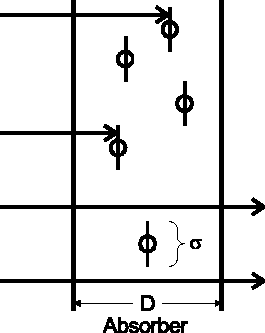
\includegraphics{figures/abb1.pdf}
    \caption{Schematische Darstellung einer Absorberschicht der Dicke $D$\cite{ap04}.}
    \label{fig:abb1}
\end{figure}

Pro Zeiteinheit finden dann, bei $N_0$ eintreffenden Teilchen,
\begin{equation}
    N = N_0 n D \sigma
    \label{eq:wechselwirkgamma}
\end{equation}
Wechselwirkungen statt. \\

Bei einem realen Absorber muss die Summation aller Schichten $\sigma$
über infinitesimale Schichten $\dif x$ stattfinden.
Nach der Integration über alle Schichten folgt daraus

\begin{equation}
    N(D) = N_0 \mathrm{e}^{-n \sigma D} \,.
    \label{eq:wechselwirkgammaexp}
\end{equation} \\

Dabei ist der Absorptionskoeffizient $\mu$ 
bei der Schichtdicke $D_{1/2}$ definiert als
\begin{equation*}
    \mu := n \sigma = D_{1/2} \ln 2 \,.
\end{equation*} \\

Zur Bestimmung der Teilchenzahl im Absorber der Ordnungszahl $\text{z}$ und
dem Molvolumen $V_{\text{Mol}}$ bzw. der Dichte $\rho$ und dem
Molekulargewicht $M$ dient
\begin{equation*}
    n = \frac{\text{z} N_A}{V_{\text{Mol}}} = \frac{\text{z} N_A \rho}{M} \,,
\end{equation*}
wobei $N_A$ die Avogadro-Konstante darstellt. \\

Der Wirkungsquerschnitt ergibt sich damit zu
\begin{equation}
    \sigma = \frac{\mu}{n} = \frac{\mu N}{z N_A \rho} \,.
    \label{eq:wirkungsquerschnitt}
\end{equation}

Jedoch stellt \eqref{eq:wirkungsquerschnitt} nur eine grobe Näherung,
keine exakte Berechnung des Wirkungsquerschnitts dar. \\


\subsubsection*{Eigenschaften der $\gamma$-Strahlung}

Geht ein Atom in einen energetisch günsigeren Zustand über, wird die
überschüssige Energie in Form von $\gamma$-Quanten abgegeben.
Diese $\gamma$-Quanten besitzen sowohl Teilchen- als auch Wellencharakter,
ihre Energie bei der Lichtgeschwindigkeit $\mathrm{c}$ ist dabei durch
\begin{equation*}
    E_\gamma = \mathrm{h} \nu = \frac{\text{h} \mathrm{c}}{\lambda}
\end{equation*}
gegeben, wobei $\nu$ die Frequenz, $\lambda$ die Wellenlänge 
und $\mathrm{h}$ das Plancksche Wirkungquantum darstellen.
Aufgrund der diskreten Kernenergieniveaus stellt das $\gamma$-Spektrum
eines Kerns ein Linienspektrum scharfer Linien dar.


\subsubsection*{Wechselwirkung mit Materie}

Dringt ein Quant in eine Materieschicht ein, kann es mit den
Elektronen, den Kernen sowie ihren elekrischen Feldern interagieren.
Die dabei möglichen Annihilationsprozesse sowie der inelastischen
und elastischen Streuung sind dabei in \autoref{fig:abb2} dargestellt.

\begin{figure}[H]
    \centering
    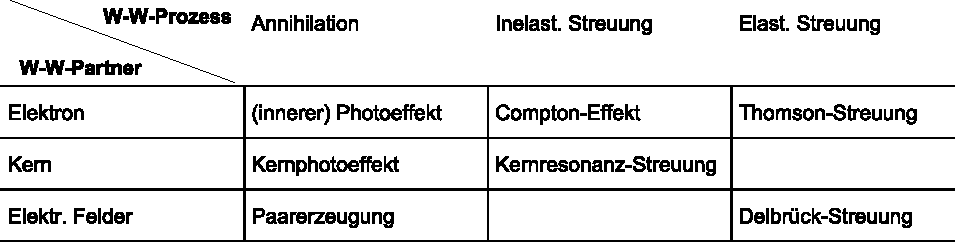
\includegraphics{figures/abb2.pdf}
    \caption{Tabellarische Darstellung der verschiedenen Wechselwirkungsmöglichkeiten von $\gamma$-Strahlung mit Materie\cite{ap04}.}
    \label{fig:abb2}
\end{figure}

Am wichtigsten sind dabei der Photoeffekt, der Comptoneffekt sowie
die Paarbildung, deren Anteile abhängig von der Energie in \autoref{fig:abb4}
dargestellt ist.

\begin{figure}[H]
    \centering
    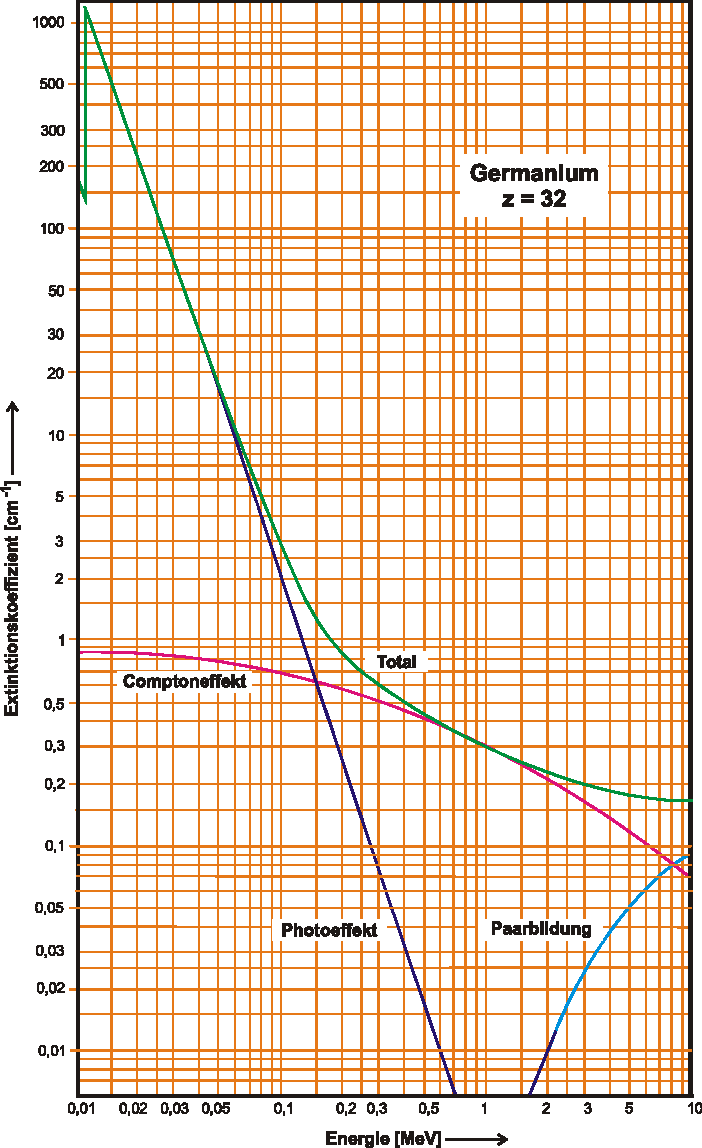
\includegraphics{figures/abb4.pdf}
    \caption{Absorptionskoeffizient $\mu$ in Abhängigkeit von der Energie am Beispiel von Germanium \cite{ap04}.}
    \label{fig:abb4}
\end{figure}

Beim Photoeffekt wechselwirkt das Photon mit einem Hüllenelektron und
wird dabei vernichtet; das Elektron wird aus seiner Bindung entfernt.
Die Elektronenenerie nach dem Stoß ist dann gegeben durch
\begin{equation*}
    E_{\mathrm{e}} = \mathrm{h} \nu - E_{\mathrm{B}} \,.
\end{equation*} \\

\begin{figure}[H]
    \centering
    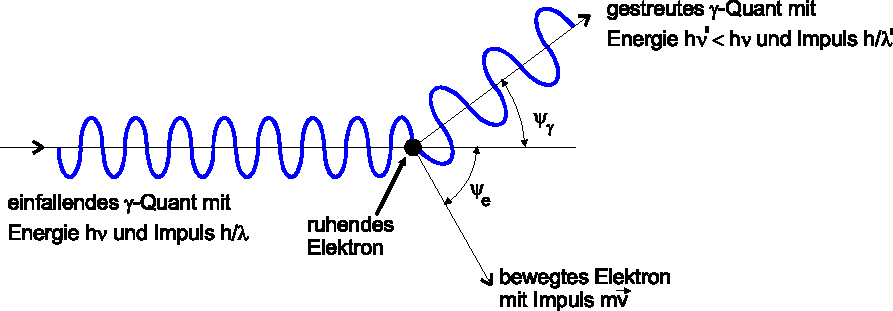
\includegraphics{figures/abb3.pdf}
    \caption{Schematische Darstellung des Comptoneffekts\cite{ap04}.}
    \label{fig:abb3}
\end{figure}

Bei der Streuung eines Quants an einem freien Elektron wird vom
Comptoneffekt gesprochen.


\autoref{fig:abb3} entsprechend gibt das Photon einen Großteil
seiner Energie an das Elektron ab, im Gegensatz zum Photoeffekt
wird das Photon aber nicht vernichtet. \\

Der Wirkungsquerschnitt $\sigma_{\mathrm{com}}$ ist dabei gegeben durch
\begin{equation}
    \sigma_{\mathrm{com}} = 2 \pi r^2_\mathrm{e} 
    \left(\frac{1 + \varepsilon}{\varepsilon^2} 
    \left[\frac{2(1 + \varepsilon)}{1 + 2 \varepsilon} -\frac{1}{\varepsilon}\right]
    + \frac{1}{2 \varepsilon} \ln(1 + 2 \varepsilon) 
    - \frac{1 + 3 \varepsilon}{(1 + 2 \varepsilon)^2}\right) \,,
    \label{eq:wirkungsquercompton}
\end{equation}
wobei $\varepsilon$ mit
\begin{equation*}
    e := \frac{E_\gamma}{m_0 c^2}
\end{equation*}
das Verhältnis der Quantenenergie $E_\gamma$ zur Ruheenergie 
des Elektrons darstellt.
Dabei ist $r_\text{e}$ der 'klassische Elektronenradius' und durch
\begin{equation*}
    r_\text{e} = \frac{\text{e}_0^2}
    {4 \pi \varepsilon_0 m_0 c^2} = 2,82 \cdot 10^{-15} \,\unit{\meter}
\end{equation*}
gegeben. \\

Nach \eqref{eq:wirkungsquerschnitt} ergibt sich der Absorptionskoeffizient
$\mu_{\text{com}}$, also der durch den Comptoneffekt bedingte
Absorptionskoeffizient, zu
\begin{equation}
    \mu_{\text{com}} = n \sigma_{\text{com}} =  
    \frac{z N_A \rho}{M} \sigma_{\text{com}} \,.
    \label{eq:absorptionskoefftheorie}
\end{equation} 

Strebt nun die Energie gegen null, ergibt sich im Grenzwert
der Thomsonsche Wirkungsquerschnitt $\sigma_{\text{Th}}$ mit

\begin{equation*}
    \lim_{\varepsilon \rightarrow 0} \sigma_{\text{com}} =
    \frac{4}{3} \cdot 2 \pi r_{\text{e}}^2 \,.
\end{equation*} \\

Ist die Energie des $\gamma$-Quants größer als die 
doppelte Ruhemasse des Elektrons, kann es im Prozess
der Paarerzeugung unter Freisetzung eines Elektrons und
Positrons vernichtet werden.
Dabei wird von einem Stoßpartner der zur Initiation der Paarbildung
fehlende Quantenimpuls übernommen.
Zumeist handelt es sich bei diesen Stoßpartnern um die 
Atomkerne des Absorbermaterials. \\

Für den Wirkungsquerschnitt der Paarbildung gilt $\sigma_{\text{p} ~ z^2}$.


\subsubsection*{Herkunft und Eigenschaften der $\beta$-Strahlung}

Je nach Zerfallsprozess wird von $\beta^+$- bzw. 
$\beta^-$-Strahlung gesprochen.

Dabei entsteht $\beta^-$-Strahlung aus
\begin{equation*}
    \text{n} \rightarrow \text{p} + \text{e}^- + \bar{\nu}_e
\end{equation*}
und $\beta^+$- Strahlung aus
\begin{equation*}
    \text{p} \rightarrow \text{n} + \text{e}^+ + \nu_e \,.
\end{equation*}

Diese Zerfälle erklären auch das in \autoref{fig:abb5} kontinuierliche Emissionsspektrum
eines $\beta$-Strahlers, da die bei der Umwandlung freiwerdende Energie
gleichmäßtig auf das Elektron/Positron und das Anti-Elektron-Neutrino/Elektron-Neutrino
verteilt.

\begin{figure}[H]
    \centering
    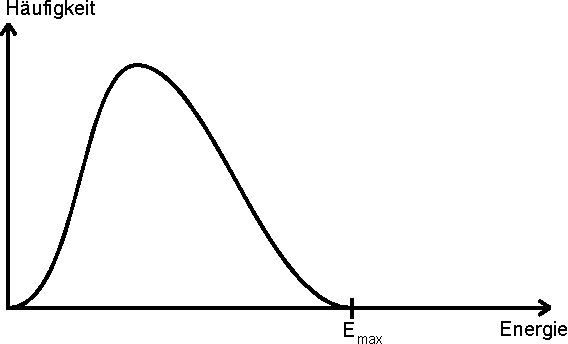
\includegraphics{figures/abb5.pdf}
    \caption{Emissionsspektrum eines $\beta$-Strahlers \cite{ap04}.}
    \label{fig:abb5}
\end{figure}


\subsubsection*{Wechselwirkung von $\beta$-Strahlung mit Materie}

Die Wechselwirkungen von $\beta$-Strahulng mit Materie lässt sich
im Grunde auf drei verschiedene Wechselwirkungen zurückführen.

\subsubsection*{Rutherford-Streuung}

Bei der Rutherford-Streuung interagieren die Elektronen mit 
den Coulombfeldern der Absorberkerne, ihre Bahnen werden stark abgelenkt,
die Strahlungsintensität des zunächst parallelen Strahls nimmt also ab,
und sie erfahren eine geringe Bremsung.

\subsection*{Bremsstrahlung}

Bei dem Eintritt in das Coulombfeld eines Atomkerns erfahren
alle geladenen Teilchen, also auch $\beta$-Teilchen, eine Beschleunigung.
Dabei muss das Teilchen Energie in Form von Strahlung abgeben, die Bremsstrahlung genannt wird. \\

Der Wirkungsquerschnitt $\sigma_{\text{Br}}$ der Bremsstrahlung lässt
sich dabei aus
\begin{equation*}
    \sigma_{\text{Br}} = \alpha r_{\text{e}}^2 z^2
\end{equation*}
berechnen.

Für die Energie, die ein $\beta$-Teilchen beim Absorberdurchgang
durch die Bremsstrahlung verliert, ergibt sich
\begin{equation*}
    E_\text{Br}[\unit{\kilo\eV}] \approx 7 \cdot 10^{-7} z E_\beta^2 \,,
\end{equation*}
wobei $E_\beta$ die Energie des einfallenden $\beta$-Teilchens beschreibt.


\subsubsection*{Ionisation und Anregung}

Streut ein $\beta$-Teilchen inelastisch an den Elektronen des
Absorbers, werden diese Elektronen angeregt oder vollständig aus dem 
Atom gelöst.
Mit der Ionisationsenergie $I$ ist der Energieverlust pro Absorberschichtdicke
gegeben durch
\begin{equation*}
    \frac{\dif E}{\dif x} \approx - \frac{2 \pi r_\text{e}^2}{E_\beta} \frac{N_A \rho}{M}
    \ln(\frac{E_\beta}{I}) \,.
\end{equation*}


\subsubsection*{Gestalt der Absorptionskurve}

Für einen Absorber der Schichtdicke $D$ ist die Massenbelegung $R$ gegeben durch
\begin{equation*}
    R = \rho D \,.
\end{equation*}

Nach einer bestimmten Massenbelegung $R_{\text{max}}$ nimmt ein
Detektor eine größtenteils schichtdickenunabhängige Intensität auf.
Um $R_\text{max}$ mit der dazugehörigen Energie $E_\text{max}$ in
Beziehung zu setzen, lässt sich

\begin{equation}
    E_\text{max} = 1,92 \sqrt{R_\text{max}^2 + 0,22 R_\text{max}}
    \label{eq:Emax}
\end{equation}
verwenden.

Eine typische Absorptionskurve ist in \autoref{fig:abb6} dargestellt.
\begin{figure}[H]
    \centering
    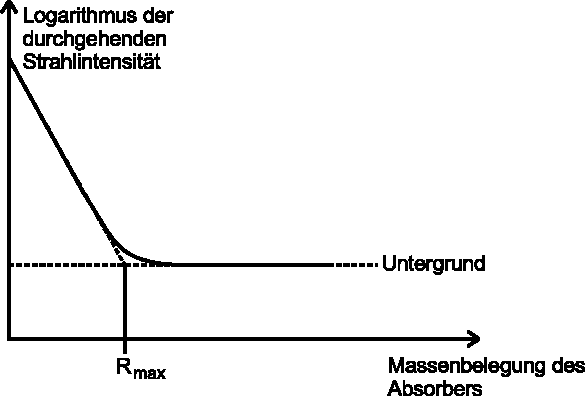
\includegraphics{figures/abb6.pdf}
    \caption{Absorptionskurve eines natürlichen $\beta$-Strahlers \cite{ap04}.}
    \label{fig:abb6}
\end{figure}
